% !Mode:: "TeX:UTF-8"
\chapter{视觉里程计2}
\begin{mdframed}  
	\textbf{主要目标}
	\begin{enumerate}[labelindent=0em,leftmargin=1.5em]
		\item 理解光流法跟踪特征点的原理。
		\item 理解直接法是如何估计相机位姿的。
		\item 使用g2o进行直接法的计算。
	\end{enumerate}
\end{mdframed}

直接法是视觉里程计另一主要分支,它与特征点法有很大不同。虽然它还没有成为现在VO中的主流,但经过近几年的发展,直接法在一定程度上已经能和特征点法平分秋色。本讲我们将介绍直接法的原理,并利用g2o实现直接法中的一些核心算法。

\newpage
\includepdf{resources/other/ch8.pdf}

\newpage
\section{直接法的引出}
上一讲我们介绍了使用特征点估计相机运动的方法。尽管特征点法在视觉里程计中占据主流地位,但研究者们还是认识到它至少有以下几个缺点:

\begin{enumerate}
	\item 关键点的提取与描述子的计算非常耗时。实践当中,SIFT目前在CPU上是无法实时计算的,而ORB也需要近20ms的计算。如果整个SLAM以30毫秒/帧的速度运行,那么一大半时间都将花在计算特征点上。
	
	\item 使用特征点时,忽略了除特征点以外的所有信息。一幅图像有几十万个像素,而特征点只有几百个。只使用特征点丢弃了大部分\textbf{可能有用的}图像信息。
	
	\item 相机有时会运动到\textbf{特征缺失}的地方,这些地方往往没有明显的纹理信息。例如,有时我们会面对一堵白墙,或者一个空荡荡的走廊。这些场景下特征点数量会明显减少,我们可能找不到足够的匹配点来计算相机运动。 
\end{enumerate}

我们看到使用特征点确实存在一些问题。有没有什么办法能够克服这些缺点呢?我们有以下几种思路:

\begin{itemize}
	\item 保留特征点,但只计算关键点,不计算描述子。同时,使用\textbf{光流法}(Optical Flow)来跟踪特征点的运动。这样可以回避计算和匹配描述子带来的时间,但光流本身的计算需要一定时间。
	\item 只计算关键点,不计算描述子。同时,使用\textbf{直接法}(Direct Method)来计算特征点在下一时刻图像中的位置。这同样可以跳过描述子的计算过程,而且直接法的计算更加简单。
	\item 既不计算关键点,也不计算描述子,而是根据像素灰度的差异,\textbf{直接}计算相机运动。
\end{itemize}

第一种方法仍然使用特征点,只是把匹配描述子替换成了光流跟踪,估计相机运动时仍使用对极几何、PnP或ICP算法。而在后两种方法中,我们会根据图像的\textbf{像素灰度信息}来计算相机运动,它们都称为\textbf{直接法}。

使用特征点法估计相机运动时,我们把特征点看作固定在三维空间的不动点。根据它们在相机中的投影位置,通过\textbf{最小化重投影误差}(Reprojection error)来优化相机运动。在这个过程中,我们需要精确地知道空间点在两个相机中投影后的像素位置——这也就是我们要对特征进行匹配或跟踪的原因。同时,我们也知道,计算、匹配特征需要付出大量的计算量。相对地,在直接法中,我们并不需要知道点与点之间的对应关系,而是通过最小化\textbf{光度误差}(Photometric error)来求得它们。

直接法是本讲介绍的重点。它是为了克服特征点法的上述缺点而存在的。直接法根据像素的亮度信息估计相机的运动,可以完全不用计算关键点和描述子,于是,既避免了特征的计算时间,也避免了特征缺失的情况。只要场景中存在明暗变化(可以是渐变,不形成局部的图像梯度),直接法就能工作。根据使用像素的数量,直接法分为稀疏、稠密和半稠密三种。相比于特征点法只能重构稀疏特征点(稀疏地图),直接法还具有恢复稠密或半稠密结构的能力。

历史上,早期也有对直接法的使用\textsuperscript{\cite{Silveira2008}}。随着一些使用直接法的开源项目的出现(如SVO\textsuperscript{\cite{Forster2014}}、LSD-SLAM\textsuperscript{\cite{Engel2014}}等),它们逐渐地走上主流舞台,成为视觉里程计算法中重要的一部分。

\section{光流(Optical Flow)}
直接法是从光流演变而来的。它们非常相似,具有相同的假设条件。光流描述了像素在图像中的运动,而直接法则附带着一个相机运动模型。为了说明直接法,我们先来介绍一下光流。

光流是一种描述像素随时间在图像之间运动的方法,如\autoref{fig:LK}~所示。随着时间的流逝,同一个像素会在图像中运动,而我们希望追踪它的运动过程。其中,计算部分像素运动的称为\textbf{稀疏光流},计算所有像素的称为\textbf{稠密光流}。稀疏光流以Lucas-Kanade光流为代表,并可以在SLAM中用于跟踪特征点位置。因此,本节主要介绍Lucas-Kanade光流,亦称LK光流。

\begin{figure}[!htp]
	\centering
	\includegraphics[width=1.0\linewidth]{vo2/opticalFlow}
	\caption{LK光流法示意图。}
	\label{fig:LK}
\end{figure}

\subsection*{Lucas-Kanade光流}
在LK光流中,我们认为来自相机的图像是随时间变化的。图像可以看作时间的函数:$\bm{I}(t)$。那么,一个在$t$时刻,位于$(x,y)$处的像素,它的灰度可以写成
\[
\bm{I}(x,y,t).
\]
这种方式把图像看成了关于位置与时间的函数,它的值域就是图像中像素的灰度。现在考虑某个固定的空间点,它在$t$时刻的像素坐标为$x,y$。由于相机的运动,它的图像坐标将发生变化。我们希望估计这个空间点在其他时刻图像中位置。怎么估计呢?这里要引入光流法的基本假设。

\textbf{灰度不变假设}:同一个空间点的像素灰度值,在各个图像中是固定不变的。

对于$t$时刻位于$(x,y)$处的像素,我们设$t+\mathrm{d}t$时刻它运动到$(x+\mathrm{d}x, y+\mathrm{d}y)$处。由于灰度不变,我们有:
\begin{equation} 
\bm{I}(x+\mathrm{d}x, y+\mathrm{d}y, t+\mathrm{d}t) = \bm{I} (x,y,t).
\end{equation}

灰度不变假设是一个很强的假设,实际当中很可能不成立。事实上,由于物体的材质不同,像素会出现高光和阴影部分;有时,相机会自动调整曝光参数,使得图像整体变亮或变暗。这些时候灰度不变假设都是不成立的,因此光流的结果也不一定可靠。然而,从另一方面来说,所有算法都是在一定假设下工作的。如果我们什么假设都不做,就没法设计实用的算法。所以,让我们暂且认为该假设成立,看看如何计算像素的运动。

对左边进行泰勒展开,保留一阶项,得:
\begin{equation}
\bm{I} \left( {x + \mathrm{d}x,y + \mathrm{d}y,t + \mathrm{d}t} \right) \approx \bm{I} \left( {x,y,t} \right) + \frac{{\partial \bm{I} }}{{\partial x}}\mathrm{d}x + \frac{{\partial \bm{I}}}{{\partial y}}\mathrm{d}y + \frac{{\partial \bm{I}}}{{\partial t}}\mathrm{d}t.
\end{equation}

因为我们假设了灰度不变,于是下一个时刻的灰度等于之前的灰度,从而:
\begin{equation}
 \frac{{\partial \bm{I} }}{{\partial x}}\mathrm{d}x + \frac{{\partial \bm{I}}}{{\partial y}}\mathrm{d}y + \frac{{\partial \bm{I}}}{{\partial t}}\mathrm{d}t = 0.
\end{equation}

两边除以$\mathrm{d}t$,得:
\begin{equation}\label{key}
 \frac{{\partial \bm{I} }}{{\partial x}} \frac{\mathrm{d}x}{\mathrm{d}t} + \frac{{\partial \bm{I}}}{{\partial y}} \frac{\mathrm{d}y}{\mathrm{d}t} =- \frac{{\partial \bm{I}}}{{\partial t}}.
\end{equation}

其中$\mathrm{d}x / \mathrm{d}t$为像素在$x$轴上的运动速度,而$\mathrm{d}y/\mathrm{d}t$为$y$轴上的速度,把它们记为$u,v$。同时$\partial \bm{I}/{\partial x}$为图像在该点处$x$方向的梯度,另一项则是在$y$方向的梯度,记为$\bm{I}_x, \bm{I}_y$。把图像灰度对时间的变化量记为$\bm{I}_t$,写成矩阵形式,有:
\begin{equation}
\left[ {\begin{array}{*{20}{c}}
	{{ \bm{I}_x}}&{{ \bm{I}_y}}
	\end{array}} \right]\left[ \begin{array}{l}
u\\
v
\end{array} \right] =  - {\bm{I}_t}.
\end{equation}

我们想计算的是像素的运动$u,v$,但是该式是带有两个变量的一次方程,仅凭它无法计算出$u,v$。因此,必须引入额外的约束来计算$u,v$。在LK光流中,我们假设\textbf{某一个窗口内的像素具有相同的运动}。

\clearpage
考虑一个大小为$w \times w$的窗口,它含有$w^2$数量的像素。由于该窗口内像素具有同样的运动,因此我们共有$w^2$个方程:
\begin{equation}
\left[ {\begin{array}{*{20}{c}}
	{{ \bm{I}_x}}&{{ \bm{I}_y}}
	\end{array}} \right]_k
\left[ \begin{array}{l}
u\\
v
\end{array} \right] =  - {\bm{I}_t}_k, \quad k=1, \ldots, w^2.
\end{equation}

记:
\begin{equation}
\bm{A} = \left[ {\begin{array}{*{20}{c}}
	{{{\left[ {{\bm{I}_x},{\bm{I}_y}} \right]}_1}}\\
	\vdots \\
	{{{\left[ {{\bm{I}_x},{\bm{I}_y}} \right]}_k}}
	\end{array}} \right],\bm{b} = \left[ {\begin{array}{*{20}{c}}
	{{ \bm{I}_{t1}}}\\
	\vdots \\
	{{ \bm{I}_{tk}}}
	\end{array}} \right].
\end{equation}

于是整个方程为
\begin{equation}
\bm{A}\left[ \begin{array}{l}
u\\
v
\end{array} \right] =  - \bm{b}.
\end{equation}

这是一个关于$u,v$的超定线性方程,传统解法是求最小二乘解。最小二乘在很多时候都用到过:
\begin{equation}
{\left[ \begin{array}{l}
	u\\
	v
	\end{array} \right]^*} = -{\left( {{ \bm{A}^\mathrm{T}}\bm{A}} \right)^{ - 1}}{ \bm{A}^\mathrm{T}}\bm{b}.
\end{equation}

这样就得到了像素在图像间的运动速度$u,v$。当$t$取离散的时刻而不是连续时间时,我们可以估计某块像素在若干个图像中出现的位置。由于像素梯度仅在局部有效,所以如果一次迭代不够好,我们会多迭代几次这个方程。在SLAM中,LK光流常被用来跟踪角点的运动,我们不妨通过程序体会一下。

\section{实践:LK光流}
\label{sec:LKFlow}
\subsection{使用TUM公开数据集}
下面演示如何用OpenCV提供的光流法来跟踪特征点。与上一节一样,我们准备了若干幅数据集图像,存放在程序目录中的data/文件夹下。它们来自于慕尼黑工业大学(TUM)提供的公开RGB-D数据集\footnote{见\url{http://vision.in.tum.de/data/datasets/rgbd-dataset/download}。}。以后我们就称之为TUM数据集。它含有许多个RGB-D视频,可以作为RGB-D或单目SLAM的实验数据。它还提供了用运动捕捉系统测量的精确轨迹,可以作为标准轨迹以校准SLAM系统。由于该数据集比较大,我们没有放到GitHub上(否则下载代码需要很长时间),请读者自行去数据集主页查找对应的数据。本程序中使用了一部分“freburg1\_desk”数据集中的图像。读者可以在TUM数据集主页找到它的下载链接。或者,也可以直接使用本书在GitHub上提供的部分。

我们的数据位于本章目录的data/下,以压缩包形式提供(data.tar.gz)。由于TUM数据集是从实际环境中采集的,需要解释一下它的数据格式(数据集一般都有自己定义的格式)。在解压后,你将看到以下这些文件:

\begin{enumerate}
	\item rgb.txt和depth.txt记录了各文件的采集时间和对应的文件名。
	\item rgb/ 和 depth/目录存放着采集到的PNG格式图像文件。彩色图像为8位3通道,深度图为16位单通道图像。文件名即采集时间。
	
	\item groundtruth.txt为外部运动捕捉系统采集到的相机位姿,格式为
	\[
	(\mathrm{time}, t_x, t_y, t_z, q_x, q_y, q_z, q_w),
	\]
	我们可以把它看成标准轨迹。
\end{enumerate}

请注意,彩色图、深度图和标准轨迹的采集都是独立的,轨迹的采集频率比图像高很多。在使用数据之前,需要根据采集时间对数据进行一次时间上的对齐,以便对彩色图和深度图进行配对。原则上,我们可以把采集时间相近于一个阈值的数据,看成是一对图像。并把相近时间的位姿,看作是该图像的真实采集位置。TUM提供了一个Python脚本“associate.py”(或使用slambook/tools/associate.py)帮我们完成这件事。请把此文件放到数据集目录下,运行:
\begin{lstlisting}[language=sh]
python associate.py rgb.txt depth.txt > associate.txt
\end{lstlisting}

这段脚本会根据输入的两个文件中的采集时间进行配对,最后输出到文件associate.txt。输出文件含有配对后的两幅图像的时间、文件名信息,可以作为后续处理的来源。此外,TUM数据集还提供了比较估计轨迹与标准轨迹的工具,我们将在用到的地方再进行介绍。

\subsection{使用LK光流}
下面来编写程序使用OpenCV中的LK光流。使用LK的目的是跟踪特征点。我们对第一幅图像提取FAST角点,然后用LK光流跟踪它们,并画在图中。

\begin{lstlisting}[language=c++,caption=slambook/ch8/useLK/useLK.cpp]
#include <iostream>
#include <fstream>
#include <list>
#include <vector>
#include <chrono>
using namespace std; 

#include <opencv2/core/core.hpp>
#include <opencv2/highgui/highgui.hpp>
#include <opencv2/features2d/features2d.hpp>
#include <opencv2/video/tracking.hpp>

int main( int argc, char** argv )
{
	if ( argc != 2 )
	{
		cout<<"usage: useLK path_to_dataset"<<endl;
		return 1;
	}
	string path_to_dataset = argv[1];
	string associate_file = path_to_dataset + "/associate.txt";
	ifstream fin( associate_file );
	string rgb_file, depth_file, time_rgb, time_depth;
	list< cv::Point2f > keypoints;      // 因为要删除跟踪失败的点,使用list
	cv::Mat color, depth, last_color;
	for ( int index=0; index<100; index++ )
	{
		fin>>time_rgb>>rgb_file>>time_depth>>depth_file;
		color = cv::imread( path_to_dataset+"/"+rgb_file );
		depth = cv::imread( path_to_dataset+"/"+depth_file, -1 );
		if (index ==0 )
		{
			// 对第一帧提取 FAST 特征点
			vector<cv::KeyPoint> kps;
			cv::Ptr<cv::FastFeatureDetector> detector = cv::FastFeatureDetector::create();
			detector->detect( color, kps );
			for ( auto kp:kps )
				keypoints.push_back( kp.pt );
			last_color = color;
			continue;
		}
        if ( color.data==nullptr || depth.data==nullptr )
	        continue;
		// 对其他帧用 LK 跟踪特征点
		vector<cv::Point2f> next_keypoints; 
		vector<cv::Point2f> prev_keypoints;
		for ( auto kp:keypoints )
			prev_keypoints.push_back(kp);
		vector<unsigned char> status;
		vector<float> error; 
		chrono::steady_clock::time_point t1 = chrono::steady_clock::now();
		cv::calcOpticalFlowPyrLK( last_color, color, prev_keypoints, next_keypoints, status, error );
		chrono::steady_clock::time_point t2 = chrono::steady_clock::now();
		chrono::duration<double> time_used = chrono::duration_cast<chrono::duration<double>>( t2-t1 );
		cout<<"LK Flow use time:"<<time_used.count()<<" seconds."<<endl;
		// 把跟丢的点删掉
		int i=0; 
		for ( auto iter=keypoints.begin(); iter!=keypoints.end(); i++)
		{
			if ( status[i] == 0 )
			{
				iter = keypoints.erase(iter);
				continue;
			}
			*iter = next_keypoints[i];
			iter++;
		}
		cout<<"tracked keypoints: "<<keypoints.size()<<endl;
		if (keypoints.size() == 0)
		{
			cout<<"all keypoints are lost."<<endl;
			break; 
		}
		// 画出 keypoints
		cv::Mat img_show = color.clone();
		for ( auto kp:keypoints )
			cv::circle(img_show, kp, 10, cv::Scalar(0, 240, 0), 1);
		cv::imshow("corners", img_show);
		cv::waitKey(0);
		last_color = color;
	}
	return 0;
}
\end{lstlisting}

读者应当已经熟悉了OpenCV的使用方式,这里就不提供CMakeLists.txt的写法了。该程序的运行参数里需要指定数据集所在的目录,例如:
\begin{lstlisting}[language=sh]
./build/useLK ../data
\end{lstlisting}

我们会在每次循环后暂停程序,按任意键可以继续运行。你会看到图像中大部分特征点都能够顺利跟踪到,但也有特征点会丢失。丢失的特征点或是被移出了视野外,或是被其他物体挡住了。如果我们不提取新的特征点,那么光流的跟踪会越来越少:

\clearpage
\begin{lstlisting}
% build/useLK ../data
LK Flow use time: 0.0329535 seconds.
tracked keypoints: 1749
LK Flow use time: 0.0247758 seconds.
tracked keypoints: 1742
LK Flow use time: 0.0226143 seconds.
tracked keypoints: 1703
LK Flow use time: 0.0238692 seconds.
tracked keypoints: 1676
LK Flow use time: 0.0210466 seconds.
tracked keypoints: 1664
LK Flow use time: 0.0226533 seconds.
tracked keypoints: 1656
LK Flow use time: 0.0266527 seconds.
tracked keypoints: 1641
LK Flow use time: 0.0214207 seconds.
tracked keypoints: 1634
\end{lstlisting}

\autoref{fig:LKFlow}~显示了程序运行过程中若干帧的情况(这里使用了完整的数据集,但本书的git上只给出了10张图)。最初我们大约有1700个特征点。跟踪过程中一部分特征点会丢失,直到100帧时我们还有约178个特征点,相机视角相对于最初的图像也发生了较大改变。

\begin{figure}[!ht]
	\centering
	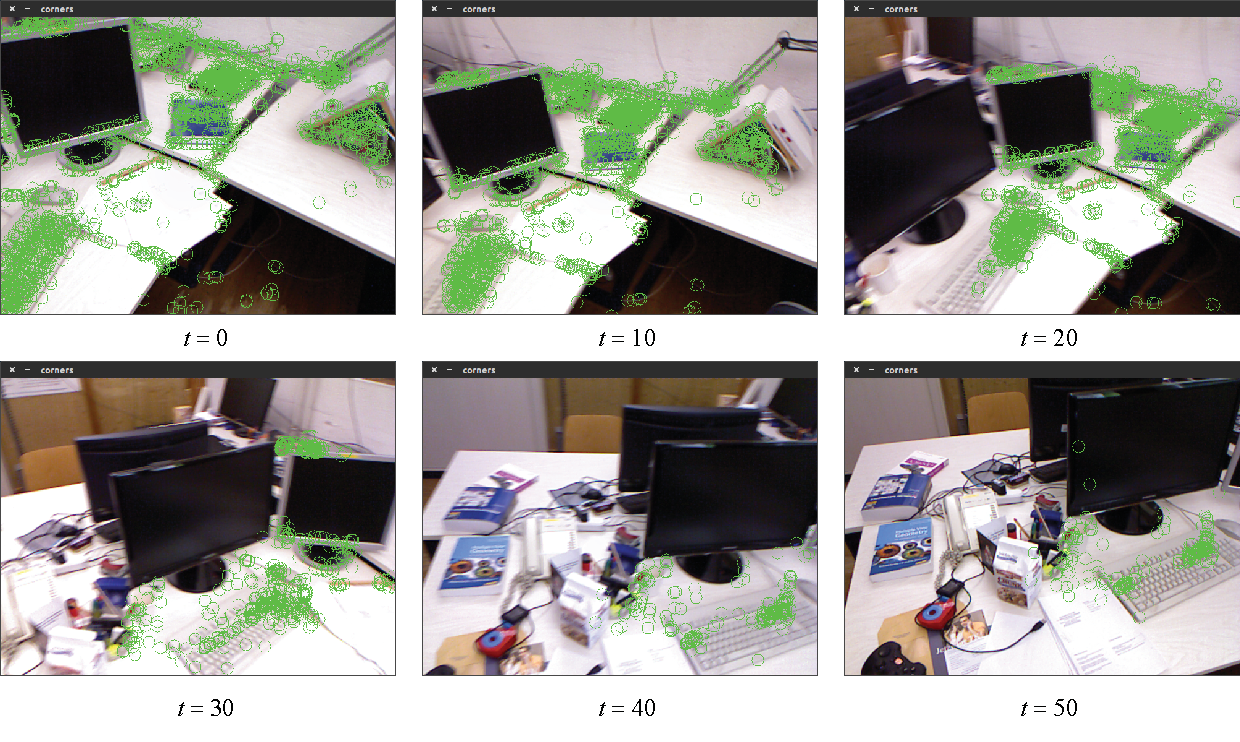
\includegraphics[width=\linewidth]{vo2/LKFlow}
	\caption{LK光流法实验。}
	\label{fig:LKFlow}
\end{figure}

仔细观察特征点的跟踪过程,我们会发现位于物体角点处的特征更加稳定。边缘处的特征会沿着边缘“滑动”,这主要是由于\textbf{沿着边缘移动时特征块的内容基本不变},因此程序容易认为是同一个地方。而既不在角点也不在边缘的特征点则会频繁跳动,位置非常不稳定。这个现象很像围棋中的“金角银边草肚皮”:角点具有更好的辨识度,边缘次之,区块最少。

另一方面,读者可以看到光流法的运行时间。在跟踪1500个特征点时,LK光流法大约需要20ms。如果减小特征点的数量,则会明显减少计算时间。我们看到,LK光流跟踪法避免了描述子的计算与匹配,但本身也需要一定的计算量。在我们的计算平台上,使用LK光流能够节省一定的计算量,但在具体SLAM系统中,使用光流还是匹配描述子,最好是亲自做实验测试一下。

另外,LK光流跟踪能够直接得到特征点的对应关系。这个对应关系就像是描述子的匹配,但实际上我们大多数时候只会碰到特征点跟丢的情况,而不太会遇到误匹配,这应该是光流相对于描述子的一点优势。但是,匹配描述子的方法在相机运动较大时仍能成功,而光流必须要求相机运动是微小的。从这方面来说,光流的健壮性比描述子差一些。

最后,我们可以通过光流跟踪的特征点,用PnP、ICP或对极几何来估计相机运动,这些方法在上一讲中介绍过,这里不再讨论。总而言之,光流法可以加速基于特征点的视觉里程计算法,避免计算和匹配描述子的过程,但要求相机运动较慢(或采集频率较高)。

\section{直接法(Direct Method)}
接下来,我们来讨论与光流有一定相似性的直接法。与前面内容相似,我们先介绍直接法的原理,然后使用g2o实现直接法。

\subsection{直接法的推导}

如\autoref{fig:directMethod}~所示,考虑某个空间点$P$和两个时刻的相机。$P$的世界坐标为$[X,Y,Z]$,它在两个相机上成像,记\textbf{非齐次}像素坐标为$\bm{p}_1, \bm{p}_2$。

\begin{figure}[!htp]
	\centering
	\includegraphics[width=.85\linewidth]{vo2/directMethod}
	\caption{直接法示意图。}
	\label{fig:directMethod}
\end{figure}

我们的目标是求第一个相机到第二个相机的相对位姿变换。我们以第一个相机为参照系,设第二个相机的旋转和平移为$\bm{R}, \bm{t}$(对应李代数为$\bm{\xi}$)。同时,两相机的内参相同,记为$\bm{K}$。为清楚起见,我们列写完整的投影方程:
\newpage
\vspace*{-2\baselineskip}
\begin{align*}
{\bm{p}_1} &= {\left[ \begin{array}{l}
	u\\
	v\\
	1
	\end{array} \right]_1} = \frac{1}{Z_1} \bm{KP}, \\
{\bm{p}_2} &= {\left[ \begin{array}{l}
	u\\
	v\\
	1
	\end{array} \right]_2} = \frac{1}{Z_2} \bm{K}\left( {\bm{RP} +\bm{t}} \right) = \frac{1}{Z_2} \bm{K} \left( \exp \left( {{\bm{\xi} ^ \wedge }} \right) {\bm{P}} \right)_{1:3}.
\end{align*}
其中$Z_1$是$P$的深度,$Z_2$是$P$在第二个相机坐标系下的深度,也就是$\bm{RP}+\bm{t}$的第3个坐标值。由于$\exp(\bm{\xi}^\wedge)$只能和齐次坐标相乘,所以我们乘完之后要取出前3个元素。这和上一讲及相机模型部分的内容是一致的。

回忆特征点法中,由于我们通过匹配描述子知道了$\bm{p}_1, \bm{p}_2$的像素位置,所以可以计算重投影的位置。但在直接法中,由于没有特征匹配,我们无从知道哪一个$\bm{p}_2$与$\bm{p}_1$对应着同一个点。直接法的思路是根据当前相机的位姿估计值来寻找$\bm{p}_2$的位置。但若相机位姿不够好,$\bm{p}_2$的外观和$\bm{p}_1$会有明显差别。于是,为了减小这个差别,我们优化相机的位姿,来寻找与$\bm{p}_1$更相似的$\bm{p}_2$。这同样可以通过解一个优化问题完成,但此时最小化的不是重投影误差,而是\textbf{光度误差}(Photometric Error),也就是$P$的两个像素的亮度误差:
\begin{equation}
e = {\bm{I}_1}\left( {{\bm{p}_1}} \right) - {\bm{I}_2}\left( {{\bm{p}_2}} \right).
\end{equation}

注意这里$e$是一个标量。同样地,优化目标为该误差的二范数,暂时取不加权的形式,为
\clearpage
\begin{equation}
\mathop {\min }\limits_{\bm{\xi}}  J\left( \bm{\xi}  \right) = \|e\|^2.
\end{equation}

能够做这种优化的理由,仍是基于\textbf{灰度不变假设}。在直接法中,我们假设一个空间点在各个视角下成像的灰度是不变的。我们有许多个(比如$N$个)空间点$P_i$,那么,整个相机位姿估计问题变为
\begin{equation}
\mathop {\min }\limits_{\bm{\xi}}  J\left( \bm{\xi}  \right) = \sum\limits_{i = 1}^N {e_i^\mathrm{T}{e_i}}, \quad {e_i} = { \bm{I}_1}\left( {{\bm{p}_{1,i}}} \right) - {\bm{I}_2}\left( {{ \bm{p}_{2,i}}} \right).
\end{equation}

注意这里的优化变量是相机位姿$\bm{\xi}$。为了求解这个优化问题,我们关心误差$e$是如何随着相机位姿$\bm{\xi}$变化的,需要分析它们的导数关系。因此,使用李代数上的扰动模型。我们给$\exp (\bm{\xi})$左乘一个小扰动$\exp( \delta \bm{\xi} )$,得:\footnote{为了避免齐次/非齐次坐标转换而导致的公式形式复杂化,我们假设中间隐式地做了所需的变化。它不会影响公式的推导。}
\begin{align*}
e\left( { \bm{\xi}  \oplus \delta \bm{\xi} } \right) &= { \bm{I} _1}\left( {\frac{1}{{{Z_1}}} \bm{KP} } \right) - {\bm{I}_2}\left( {\frac{1}{{{Z_2}}} \bm{K}\exp \left( {\delta {\bm{\xi} ^ \wedge }} \right)\exp \left( {{\bm{\xi} ^ \wedge }} \right) {\bm{P}}} \right)\\
& \approx {\bm{I}_1}\left( {\frac{1}{{{Z_1}}} \bm{KP}} \right) - {\bm{I}_2}\left( {\frac{1}{{{Z_2}}} \bm{K} \left( {1 + \delta {\bm{\xi} ^ \wedge }} \right)\exp \left( {{ \bm{\xi} ^ \wedge }} \right) {\bm{P}} } \right)\\
&= {\bm{I}_1}\left( {\frac{1}{{{Z_1}}} \bm{KP}} \right) - {\bm{I}_2}\left( {\frac{1}{{{Z_2}}} \bm{K}\exp \left( {{\bm{\xi} ^ \wedge }} \right) \bm{P} + \frac{1}{{{Z_2}}} \bm{K} \delta { \bm{\xi} ^ \wedge }\exp \left( {{\bm{\xi} ^ \wedge }} \right) {\bm{P}}} \right).
\end{align*}

类似于上一讲,记:
\begin{align*}
\bm{q} &= \delta \bm{\xi} ^\wedge \exp \left( {{ \bm{\xi} ^ \wedge }} \right) \bm{P}, \\
\bm{u} &= \frac{1}{{{Z_2}}} \bm{K} \bm{q}.
\end{align*}

这里的$\bm{q}$为扰动分量在第二个相机坐标系下的坐标,而$\bm{u}$为它的像素坐标。利用一阶泰勒展开,有:
\begin{align*}
e \left( { \bm{\xi}  \oplus \delta \bm{\xi} } \right) &= {\bm{I}_1}\left( {\frac{1}{{{Z_1}}} \bm{KP}} \right) - {\bm{I}_2}\left( {\frac{1}{{{Z_2}}} \bm{K} \exp \left( {{\bm{\xi} ^ \wedge }} \right) \bm{P} + \bm{u}} \right)\\
& \approx { \bm{I}_1}\left( {\frac{1}{{{Z_1}}} \bm{KP}} \right) - {\bm{I}_2}\left( {\frac{1}{{{Z_2}}} \bm{K}\exp \left( {{\bm{\xi} ^ \wedge }} \right) \bm{P}} \right) - \frac{{\partial { \bm{I}_2}}}{{\partial \bm{u}}}\frac{{\partial \bm{u}}}{{\partial \bm{q}}}\frac{{\partial \bm{q}}}{{\partial \delta \bm{\xi} }}\delta \bm{\xi} \\
&= e\left( \bm{\xi}  \right) - \frac{{\partial {\bm{I}_2}}}{{\partial \bm{u}}}\frac{{\partial \bm{u}}}{{\partial \bm{q}}}\frac{{\partial \bm{q}}}{{\partial \delta \bm{\xi} }}\delta \bm{\xi} .
\end{align*}

\clearpage
我们看到,一阶导数由于链式法则分成了3项,而这3项都是容易计算的:

\begin{enumerate}
	\item $ \partial \bm{I}_2 / \partial \bm{u} $ 为$\bm{u}$处的像素梯度。
	\item $ \partial \bm{u} / \partial \bm{q} $ 为投影方程关于相机坐标系下的三维点的导数。记$\bm{q}=[X,Y,Z]^\mathrm{T}$,根据上一节的推导,导数为
	\begin{equation}
	\frac{{\partial \bm{u}}}{{\partial \bm{q}}} = \left[ {\begin{array}{*{20}{c}}
		{\frac{{\partial u}}{{\partial X}}}&{\frac{{\partial u}}{{\partial Y}}}&{\frac{{\partial u}}{{\partial Z}}}\\
		{\frac{{\partial v}}{{\partial X}}}&{\frac{{\partial v}}{{\partial Y}}}&{\frac{{\partial v}}{{\partial Z}}}
		\end{array}} \right] = \left[ {\begin{array}{*{20}{c}}
		{\frac{{{f_x}}}{{\rm{Z}}}}&0&{ - \frac{{{f_x}X}}{{{Z^2}}}}\\
		0&{\frac{{{f_y}}}{Z}}&{ - \frac{{{f_y}Y}}{{{Z^2}}}}
		\end{array}} \right].
	\end{equation}
	
	\item ${\partial \bm{q}}/{\partial \delta \bm{\xi} }$为变换后的三维点对变换的导数,这在李代数一讲介绍过了:
	\begin{equation}
	\frac{{\partial \bm{q}}}{{\partial \delta \bm{\xi} }} = \left[ { \bm{I}, - {\bm{q}^ \wedge }} \right].
	\end{equation}
\end{enumerate}

在实践中,由于后两项只与三维点$\bm{q}$有关,而与图像无关,我们经常把它合并在一起:
\begin{equation}
\frac{{\partial \bm{u}}}{{\partial \delta \bm{\xi} }} = \left[ {\begin{array}{*{20}{c}}
	{\frac{{{f_x}}}{Z}}&0&{ - \frac{{{f_x}X}}{{{Z^2}}}}&{ - \frac{{{f_x}XY}}{{{Z^2}}}}&{{f_x} + \frac{{{f_x}{X^2}}}{{{Z^2}}}}&{ - \frac{{{f_x}Y}}{Z}}\\
	0&{\frac{{{f_y}}}{Z}}&{ - \frac{{{f_y}Y}}{{{Z^2}}}}&{ - {f_y} - \frac{{{f_y}{Y^2}}}{{{Z^2}}}}&{\frac{{{f_y}XY}}{{{Z^2}}}}&{\frac{{{f_y}X}}{Z}}
	\end{array}} \right].
\end{equation}

这个$2 \times 6$的矩阵在上一讲中也出现过。于是,我们推导出误差相对于李代数的雅可比矩阵:
\begin{equation}
\label{eq:jacobianofDirect}
\bm{J} =  - \frac{{\partial { \bm{I}_2}}}{{\partial \bm{u}}}\frac{{\partial \bm{u}}}{{\partial \delta \bm{\xi} }}.
\end{equation}

对于$N$个点的问题,我们可以用这种方法计算优化问题的雅可比矩阵,然后使用高斯牛顿法或列文伯格—马夸尔特方法计算增量,迭代求解。至此,我们推导了直接法估计相机位姿的整个流程,下面通过程序来演示一下直接法是如何使用的。

\subsection{直接法的讨论}
在上面的推导中,$P$是一个已知位置的空间点,它是怎么来的呢?在RGB-D相机下,我们可以把任意像素反投影到三维空间,然后投影到下一幅图像中。如果在单目相机中,这件事情要更为困难,因为我们还须考虑由$P$的深度带来的不确定性。详细的深度估计放到第13讲中讨论。现在我们先来考虑简单的情况,即$P$深度已知的情况。

根据$P$的来源,我们可以把直接法进行分类:
\begin{enumerate}
	\item $P$来自于稀疏关键点,我们称之为稀疏直接法。通常我们使用数百个至上千个关键点,并且像L-K光流那样,假设它周围像素也是不变的。这种稀疏直接法不必计算描述子,并且只使用数百个像素,因此速度最快,但只能计算稀疏的重构。
\clearpage
	\item $P$来自部分像素。我们看到式\eqref{eq:jacobianofDirect}中,如果像素梯度为零,整项雅可比矩阵就为零,不会对计算运动增量有任何贡献。因此,可以考虑只使用带有梯度的像素点,舍弃像素梯度不明显的地方。这称为半稠密(Semi-Dense)的直接法,可以重构一个半稠密结构。
	\item $P$为所有像素,称为稠密直接法。稠密重构需要计算所有像素(一般几十万至几百万个),因此多数不能在现有的CPU上实时计算,需要GPU的加速。但是,如前面所讨论的,像素梯度不明显的点,在运动估计中不会有太大贡献,在重构时也会难以估计位置。
\end{enumerate}

可以看到,从稀疏到稠密重构,都可以用直接法来计算。它们的计算量是逐渐增长的。稀疏方法可以快速地求解相机位姿,而稠密方法可以建立完整地图。具体使用哪种方法,需要视机器人的应用环境而定。特别地,在低端的计算平台上,稀疏直接法可以做到非常快速的效果,适用于实时性较高且计算资源有限的场合\textsuperscript{\cite{Engel2016}}。

\section{实践:RGB-D的直接法}
\subsection{稀疏直接法}
现在,我们来演示如何使用稀疏的直接法。由于本书不涉及GPU编程,稠密的直接法就省略掉了。同时,为了保持程序简单,我们使用RGB-D数据而非单目数据,这样可以省略掉单目的深度恢复部分。基于特征点的深度恢复已经在上一讲介绍过,而基于块匹配的深度恢复将在后面介绍。所以本节我们来考虑RGB-D上的稀疏直接法VO。

由于求解直接法最后等价于求解一个优化问题,因此可以使用g2o或Ceres这些优化库来帮助求解。本节以g2o为例设计实验,而Ceres部分则留作习题。在使用g2o之前,需要把直接法抽象成一个图优化问题。显然,直接法是由以下顶点和边组成的:

\begin{enumerate}
	\item 优化变量为一个相机位姿,因此需要一个位姿顶点。由于我们在推导中使用了李代数,故程序中使用李代数表达的$\mathrm{SE}(3)$位姿顶点。与上一讲一样,我们将使用“VertexSE3Expmap”作为相机位姿。
	\item 误差项为单个像素的光度误差。由于整个优化过程中$\bm{I}_1(\bm{p}_1)$保持不变,我们可以把它当成一个固定的预设值,然后调整相机位姿,使$\bm{I}_2(\bm{p}_2)$接近这个值。于是,这种边只连接一个顶点,为\textbf{一元边}。由于g2o中本身没有计算光度误差的边,我们需要自己定义一种新的边。
\end{enumerate}

在上述的建模中,直接法图优化问题是由一个相机位姿顶点与许多条一元边组成的。如果使用稀疏的直接法,那我们大约会有几百至几千条这样的边;稠密直接法则会有几十万条边。优化问题对应的线性方程是计算李代数增量,本身规模不大(6$\times$6),所以主要的计算时间会花费在每条边的误差与雅可比矩阵的计算上。下面的实验中,我们先来定义一种用于直接法位姿估计的边,然后,使用该边构建图优化问题并求解。

\subsection{定义直接法的边}
首先定义计算光度误差的边。按照前面的推导,还需要给出它的雅可比矩阵:

\begin{lstlisting}[language=c++,caption=slambook/ch8/directMethod/direct\_sparse.cpp(片段)]
// project a 3d point into an image plane, the error is photometric error
// an unary edge with one vertex SE3Expmap (the pose of camera)
class EdgeSE3ProjectDirect: public BaseUnaryEdge< 1, double, VertexSE3Expmap>
{
public:
	EIGEN_MAKE_ALIGNED_OPERATOR_NEW
	
	EdgeSE3ProjectDirect() {}
	
	EdgeSE3ProjectDirect ( Eigen::Vector3d point, float fx, float fy, float cx, float cy, cv::Mat* image ) : x_world_ ( point ), fx_ ( fx ), fy_ ( fy ), cx_ ( cx ), cy_ ( cy ), image_ ( image )
	{}
	
	virtual void computeError()
	{
		const VertexSE3Expmap* v  =static_cast<const VertexSE3Expmap*> ( _vertices[0] );
		Eigen::Vector3d x_local = v->estimate().map ( x_world_ );
		float x = x_local[0]*fx_/x_local[2] + cx_;
		float y = x_local[1]*fy_/x_local[2] + cy_;
		// check x,y is in the image
		if ( x-4<0 || ( x+4 ) >image_->cols || ( y-4 ) <0 || ( y+4 ) >image_->rows )
		{
			_error ( 0,0 ) = 0.0;
			this->setLevel ( 1 );
		}
		else
		{
			_error ( 0,0 ) = getPixelValue ( x,y ) - _measurement;
		}
	}

	// plus in manifold
	virtual void linearizeOplus( )
	{
	     if ( level() == 1 )
	     {
		     _jacobianOplusXi = Eigen::Matrix<double, 1, 6>::Zero();
		     return;
	     }
		VertexSE3Expmap* vtx = static_cast<VertexSE3Expmap*> ( _vertices[0] );
		Eigen::Vector3d xyz_trans = vtx->estimate().map ( x_world_ );   // q in book
		
		double x = xyz_trans[0];
		double y = xyz_trans[1];
		double invz = 1.0/xyz_trans[2];
		double invz_2 = invz*invz;
		
		float u = x*fx_*invz + cx_;
		float v = y*fy_*invz + cy_;
		
		// jacobian from se3 to u,v
		// NOTE that in g2o the Lie algebra is (\omega, \epsilon), where \omega is so(3) and \epsilon the translation
		Eigen::Matrix<double, 2, 6> jacobian_uv_ksai;
		
		jacobian_uv_ksai ( 0,0 ) = - x*y*invz_2 *fx_;
		jacobian_uv_ksai ( 0,1 ) = ( 1+ ( x*x*invz_2 ) ) *fx_;
		jacobian_uv_ksai ( 0,2 ) = - y*invz *fx_;
		jacobian_uv_ksai ( 0,3 ) = invz *fx_;
		jacobian_uv_ksai ( 0,4 ) = 0;
		jacobian_uv_ksai ( 0,5 ) = -x*invz_2 *fx_;
		
		jacobian_uv_ksai ( 1,0 ) = - ( 1+y*y*invz_2 ) *fy_;
		jacobian_uv_ksai ( 1,1 ) = x*y*invz_2 *fy_;
		jacobian_uv_ksai ( 1,2 ) = x*invz *fy_;
		jacobian_uv_ksai ( 1,3 ) = 0;
		jacobian_uv_ksai ( 1,4 ) = invz *fy_;
		jacobian_uv_ksai ( 1,5 ) = -y*invz_2 *fy_;
		
		Eigen::Matrix<double, 1, 2> jacobian_pixel_uv;
		
		jacobian_pixel_uv ( 0,0 ) = ( getPixelValue ( u+1,v )-getPixelValue ( u-1,v ) ) /2;
		jacobian_pixel_uv ( 0,1 ) = ( getPixelValue ( u,v+1 )-getPixelValue ( u,v-1 ) ) /2;
		
		_jacobianOplusXi = jacobian_pixel_uv*jacobian_uv_ksai;
	}

	// dummy read and write functions because we don't care...
	virtual bool read ( std::istream& in ) {}
	virtual bool write ( std::ostream& out ) const {}

protected:
	// get a gray scale value from reference image (bilinear interpolated)
	inline float getPixelValue ( float x, float y )
	{
		uchar* data = & image_->data[ int ( y ) * image_->step + int ( x ) ];
		float xx = x - floor ( x );
		float yy = y - floor ( y );
		return float (
			( 1-xx ) * ( 1-yy ) * data[0] +
			xx* ( 1-yy ) * data[1] +
			( 1-xx ) *yy*data[ image_->step ] +
			xx*yy*data[image_->step+1]
		);
	}
public:
	Eigen::Vector3d x_world_;   // 3D point in world frame
	float cx_=0, cy_=0, fx_=0, fy_=0; // Camera intrinsics
	cv::Mat* image_=nullptr;    // reference image
};
\end{lstlisting}

我们的边继承自g2o::BaseUnaryEdge。在继承时,需要在模板参数里填入测量值的维度、类型,以及连接此边的顶点,同时,我们把空间点$P$、相机内参和图像存储在该边的成员变量中。为了让g2o优化该边对应的误差,我们需要覆写两个虚函数:用computeError()计算误差值,用linearizeOplus()计算雅可比矩阵。可以看到,这里的雅可比矩阵计算与式\eqref{eq:jacobianofDirect}是一致的。注意我们在程序中的误差计算里使用了$\bm{I}_2(\bm{p}_2) - \bm{I}_1(\bm{p}_1)$的形式,因此前面的负号可以省去,只需把像素梯度乘以像素到李代数的梯度即可。

在程序中,相机位姿是用浮点数表示的,投影到像素坐标也是浮点形式。为了更精细地计算像素亮度,我们要对图像进行插值。我们这里采用了简单的双线性插值,也可以使用更复杂的插值方式,但计算代价可能会变高一些。

\subsection{使用直接法估计相机运动}
定义了g2o边后,我们将节点和边组合成图,就可以调用g2o进行优化了。实现代码位于slambook/ch8/directMethod/direct\_sparse.cpp中,请读者阅读该部分代码并编译。

在这个实验中,我们读取数据集的RGB-D图像序列。以第一幅图像为参考帧,然后用直接法求解后续图像的位姿。在参考帧中,对第一幅图像提取FAST关键点(不需要描述子),并使用直接法估计这些关键点在第二幅图像中的位置,以及第二幅图像的相机位姿。这就构成了一种简单的稀疏直接法。最后,我们画出这些关键点在第二幅图像中的投影。

执行如下命令:
\begin{lstlisting}[language=sh]
build/direct_sparse ~/dataset/rgbd_dataset_freiburg1_desk
\end{lstlisting}

程序会在作图之后暂停,你可以看到特征点的位置关系,终端也会输出迭代误差的下降过程。

如\autoref{fig:directExperiment2}~所示,我们看到在两幅图像相差不多时,直接法会调整相机的位姿,使得大部分像素都能够正确跟踪。但是,在稍长一点的时间内,比如说0\textasciitilde9帧之间的对比,我们发现由于相机位姿估计不准确,特征点出现了明显的偏移现象。我们会在本讲末尾对其进行分析。

\begin{figure}[!htp]
	\centering
	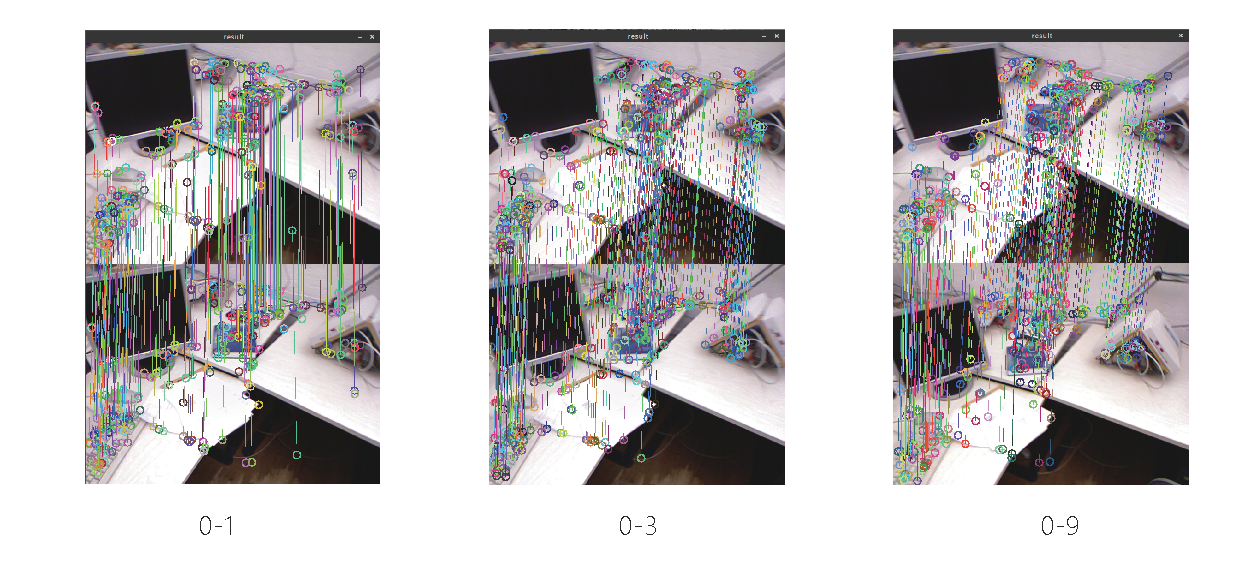
\includegraphics[width=1.0\linewidth]{vo2/directExperiment2}
	\caption{稀疏直接法的实验。左:误差随着迭代下降。右:参考帧与后1\textasciitilde9帧对比(选取部分关键点)。}
	\label{fig:directExperiment2}
\end{figure}

\subsection{半稠密直接法}
我们很容易就能把程序拓展成半稠密的直接法形式。对参考帧,先提取梯度较明显的像素,然后用直接法,以这些像素为图优化边来估计相机运动。对先前的程序做如下修改:

\begin{lstlisting}[language=c++,caption=slambook/ch8/direct\_semidense.cpp]
// select the pixels with high gradiants 
for ( int x=10; x<gray.cols-10; x++ )
	for ( int y=10; y<gray.rows-10; y++ )
	{
		Eigen::Vector2d delta (
			gray.ptr<uchar>(y)[x+1] - gray.ptr<uchar>(y)[x-1], 
			gray.ptr<uchar>(y+1)[x] - gray.ptr<uchar>(y-1)[x]
		);
		if ( delta.norm() < 50 )
			continue;
		ushort d = depth.ptr<ushort> (y)[x];
		if ( d==0 )
			continue;
		Eigen::Vector3d p3d = project2Dto3D ( x, y, d, fx, fy, cx, cy, depth_scale );
		float grayscale = float ( gray.ptr<uchar> (y) [x] );
		measurements.push_back ( Measurement ( p3d, grayscale ) );
	}
\end{lstlisting}

这只是一个很简单的改动。我们把先前的稀疏特征点改成了带有明显梯度的像素。于是在图优化中会增加许多的边。这些边都会参与估计相机位姿的优化问题,利用大量的像素而不单单是稀疏的特征点。由于我们并没有使用所有的像素,所以这种方式又称为\textbf{半稠密方法(Semi-dense)}。我们把参与估计的像素取出来并在图像中显示出来,如\autoref{fig:direct-semidense}~所示。

\begin{figure}[!htp]
	\centering
	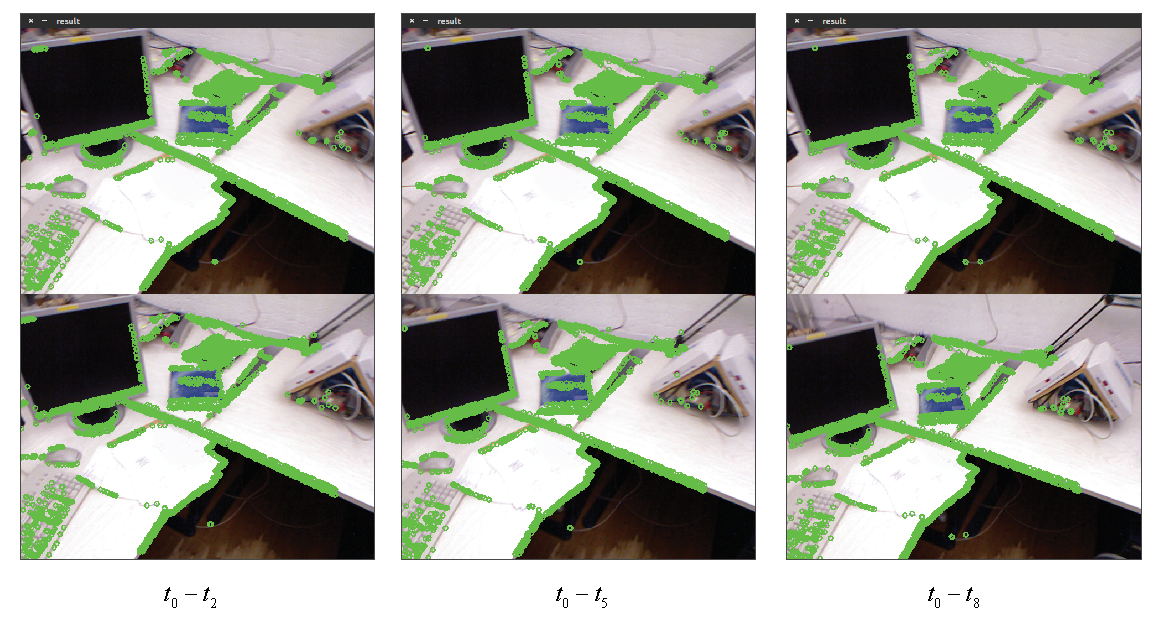
\includegraphics[width=1.0\linewidth]{vo2/direct-semidense.pdf}
	\caption{半稠密直接法的实验。参考帧与第2, 5, 8帧的对比,绿色部分标出了参与优化的像素。}
	\label{fig:direct-semidense}
\end{figure}

如果读者亲自做了实验,就可以看到参与估计的像素像是\textbf{固定在空间中一样}。当相机旋转时,它们的位置似乎没有发生变化。这代表了我们估计的相机运动是正确的。同时,你可以检查使用的像素数量与优化时间的关系。显然,当像素增多时,优化会更加费时,所以为了实时性,需要考虑使用较好的像素点,或者降低图像的分辨率。不过对于演示实验来说,笔者认为这样已经能够理解直接法的意义了。

\clearpage
\subsection{直接法的讨论}
相比于特征点法,直接法完全依靠优化来求解相机位姿。从式\eqref{eq:jacobianofDirect}中可以看到,像素梯度引导着优化的方向。如果想要得到正确的优化结果,就必须保证\textbf{大部分像素梯度能够把优化引导到正确的方向}。

这是什么意思呢?我们不妨设身处地地扮演一下优化算法。假设对于参考图像,我们测量到一个灰度值为229的像素。并且,由于我们知道它的深度,可以推断出空间点$P$的位置(\autoref{fig:directExperiment}~所示在$I_1$中测量到的灰度)。

\begin{figure}[!htp]
	\centering
	\includegraphics[width=.9\linewidth]{vo2/directExperiment}
	\caption{一次迭代的图形化显示。}
	\label{fig:directExperiment}
\end{figure}

此时我们又得到了一幅新的图像,需要估计它的相机位姿。这个位姿是由一个初值不断地优化迭代得到的。假设我们的初值比较差,在这个初值下,空间点$P$投影后的像素灰度值是126。于是,这个像素的误差为$229-126=103$。为了减小这个误差,我们希望\textbf{微调相机的位姿,使像素更亮一些}。

怎么知道往哪里微调像素会更亮呢?这就需要用到局部的像素梯度。我们在图像中发现,沿$u$轴往前走一步,该处的灰度值变成了123,即减去了3。同样地,沿$v$轴往前走一步,灰度值减了18,变成108。在这个像素周围,我们看到梯度是$[-3,-18]$,为了提高亮度,我们会建议优化算法微调相机,使$P$的像往\textbf{左上方}移动。在这个过程中,我们用像素的局部梯度近似了它附近的灰度分布,不过请注意,真实图像并不是光滑的,所以这个梯度在远处就不成立了。

但是,优化算法不能只听这个像素的一面之词,还需要听取其他像素的建议\footnote{这可能是一种不严谨的拟人化说法,不过有助于理解。}。综合听取了许多像素的意见之后,优化算法选择了一个和我们建议的方向偏离不远的地方,计算出一个更新量$\exp ({\bm{\xi}^\wedge } )$。加上更新量后,图像从$I_2$移动到了$I_2'$,像素的投影位置也变到了一个更亮的地方。我们看到,通过这次更新,\textbf{误差变小了}。在理想情况下,我们期望误差会不断下降,最后收敛。

但是实际是不是这样呢?我们是否真的只要沿着梯度方向走,就能走到一个最优值?注意到,直接法的梯度是直接由图像梯度确定的,因此我们必须保证\textbf{沿着图像梯度走时,灰度误差会不断下降}。然而,图像通常是一个很强烈的\textbf{非凸函数},如\autoref{fig:non-convex}~所示。实际当中,如果我们沿着图像梯度前进,很容易由于图像本身的非凸性(或噪声)落进一个局部极小值中,无法继续优化。只有当相机运动很小,图像中的梯度不会有很强的非凸性时,直接法才能成立。

\begin{figure}[!htp]
	\centering
	\includegraphics[width=1.0\linewidth]{vo2/nonconvex}
	\caption{一张图像的三维化显示。从图像中的一个点运动到另一个点的路径不见得是“笔直的下坡路”,而需要经常“翻山越岭”。这体现了图像本身的非凸性。}
	\label{fig:non-convex}
\end{figure}

在例程中,我们只计算了单个像素的差异,并且这个差异是由灰度直接相减得到的。然而,单个像素没有什么区分性,周围很可能有好多像素和它的亮度差不多。所以,我们有时会使用小的图像块(patch),并且使用更复杂的差异度量方式,例如归一化相关性(Normalized Cross Correlation,NCC)等(见第13讲)。而例程为了简单起见,使用了误差的平方和,以保持与推导的一致性。

\subsection{直接法优缺点总结}
最后,我们总结一下直接法的优缺点。大体上,它的优点如下:

\begin{itemize}
	\item 可以省去计算特征点、描述子的时间。
	\item 只要求有像素梯度即可,不需要特征点。因此,直接法可以在特征缺失的场合下使用。比较极端的例子是只有渐变的一幅图像。它可能无法提取角点类特征,但可以用直接法估计它的运动。
	\item 可以构建半稠密乃至稠密的地图,这是特征点法无法做到的。
\end{itemize}

另一方面,它的缺点也很明显:
\begin{itemize}
	\item \textbf{非凸性}。直接法完全依靠梯度搜索,降低目标函数来计算相机位姿。其目标函数中需要取像素点的灰度值,而图像是强烈非凸的函数。这使得优化算法容易进入极小,只在运动很小时直接法才能成功。
	\item \textbf{单个像素没有区分度}。和它像的实在太多了!于是我们要么计算图像块,要么计算复杂的相关性。由于每个像素对改变相机运动的“意见”不一致,只能少数服从多数,以数量代替质量。
	\item \textbf{灰度值不变是很强的假设}。如果相机是自动曝光的,当它调整曝光参数时,会使得图像整体变亮或变暗。光照变化时亦会出现这种情况。特征点法对光照具有一定的容忍性,而直接法由于计算灰度间的差异,整体灰度变化会破坏灰度不变假设,使算法失败。针对这一点,目前的直接法开始使用更细致的光度模型标定相机,以便在曝光时间变化时也能工作。
\end{itemize}

\section*{习题}
\begin{enumerate}
	\item 除了LK光流之外,还有哪些光流方法?它们各有什么特点?
	\item 在本节程序的求图像梯度过程中,我们简单地求了$u+1$和$u-1$的灰度之差除以2,作为$u$方向上的梯度值。这种做法有什么缺点?提示:对于距离较近的特征,变化应该较快;而距离较远的特征在图像中变化较慢,求梯度时能否利用此信息?
	\item 在稀疏直接法中,假设单个像素周围小块的光度也不变,是否可以提高算法健壮性?请编程实现。
	\item[\optional] 使用Ceres实现RGB-D上的稀疏直接法和半稠密直接法。
	\item 相比于RGB-D的直接法,单目直接法往往更加复杂。除了匹配未知之外,像素的距离也是待估计的,我们需要在优化时把像素深度也作为优化变量。阅读文献\cite{Engel2013, Engel2014},你能理解它的原理吗?如果不能,请在第13讲后再回来阅读。
	\item 由于图像的非凸性,直接法目前还只能用于短距离、非自动曝光的相机。你能否提出增强直接法健壮性的方案?阅读文献\cite{Engel2016, Usenko2016}可能会给你一些灵感。
\end{enumerate}


